% !TeX spellcheck = en_US
\documentclass[usenames, dvipsnames, aspectratio = 169]{beamer}
\setbeamertemplate{navigation symbols}{}

\usepackage{mathtools, cases, graphicx, xcolor, graphics, mathrsfs, dsfont, amssymb, multirow, dcolumn, natbib, hyperref, multicol, subcaption, changepage, booktabs, caption, appendixnumberbeamer, enumerate, natbib}
\usepackage{lmodern} % http://ctan.org/pkg/lm
\usepackage{textpos}
\usepackage{tikz}
\usepackage{transparent}
\usepackage{dcolumn}
\usepackage{tabularx}
\usepackage[flushleft]{threeparttable}
\usepackage[utf8]{inputenc}
\usepackage[T1]{fontenc}
\usetheme{Boadilla}

\usetikzlibrary{calc}
\newcommand{\tikzmark}[1]{\tikz[overlay,remember picture] \node (#1) {};}
\newcommand{\DrawBox}[3][]{%
    \tikz[overlay,remember picture]{
    \draw[black,#1]
      ($(#2)+(-0.5em,2.0ex)$) rectangle
      ($(#3)+(9em,-0.75ex)$);}
}

% AMSMATH : theorems environments
\setbeamertemplate{theorems}[numbered]
% \newtheorem{theorem}{Theorem}
\newtheorem{assumption}{Assumption}
% \newtheorem{corollary}[theorem]{Corollary}
\newtheorem{proposition}{Proposition}
% \newtheorem{lemma}[theorem]{Lemma}
\newtheorem{conjecture}{Conjecture}
% \newenvironment{proof}[1][Proof]{\noindent\textbf{#1.} }{\ \rule{0.5em}{0.5em}}

% Define University colors
\definecolor{OrangeAMSE}{HTML}{f1ae0f}
\definecolor{BlueAMSE}{HTML}{0563bc}
% Set color for structure
\setbeamercolor{structure}{fg = BlueAMSE, bg = OrangeAMSE}

% HYPERREF : Hyperlink colors
\hypersetup{
	colorlinks = true,
	linkcolor = white,
	anchorcolor = blue,
	citecolor = OrangeAMSE!75,
	filecolor = blue,
	urlcolor = OrangeAMSE!75
}

\setcounter{tocdepth}{2}
% \setbeamertemplate{sections/subsections in toc}[sections numbered]
\setbeamertemplate{section in toc}{\hspace*{1em}\inserttocsection}
\setbeamertemplate{enumerate items}[default]
\setbeamertemplate{itemize items}[square]
\setbeamertemplate{itemize subitem}[default]
\setbeamercovered{transparent}

\useoutertheme[footline=empty, subsection=false]{miniframes}

\setbeamercolor{section in head/foot}{fg=white, bg=structure.fg!75}
\setbeamercolor*{mini frame}{fg=white, bg=white}
\setbeamercolor{page number in head/foot}{fg=white}
\setbeamercolor{date in head/foot}{fg=white}
\setbeamercolor{lower separation line head}{bg = OrangeAMSE!75}

\setbeamercolor{section in toc}{fg=BlueAMSE}
\setbeamercolor{emph}{fg=BlueAMSE}
\renewcommand<>{\emph}[1]{%
  {\usebeamercolor[fg]{emph}#1}%
}

\begin{document}
	\title[Essays on inter-generational dynamics in Economics]{Essays on inter-generational dynamics in Economics}
	\author[Fabien Petit]{Fabien Petit}
	\institute[AMSE]{Aix-Marseille University, CNRS, AMSE}
	\date{May 6, 2022}
	
	\begin{frame}[plain]
		\titlepage
		\vspace{-0.5cm}
    	\begin{center}
    	    \href{https://www.fabienpetit.com}{www.fabienpetit.com} {\color{OrangeAMSE}|} \href{mailto:fabien.petit@univ-amu.fr}{fabien.petit@univ-amu.fr}
    	\end{center}
		\begin{figure}
			\begin{subfigure}[h]{0.49\linewidth}
				\centering
				
\includegraphics[width=0.5\linewidth]{logo/amu.png} 
			\end{subfigure}
			%%%
			\begin{subfigure}[h]{0.49\linewidth}
				\centering
				
\includegraphics[width=0.5\linewidth]{logo/amse.png}
			\end{subfigure}
		\end{figure}
	\end{frame}

\renewcommand{\thesection}{}

\section{Introduction}
\begin{frame}{What generation are you?}
    \begin{figure}
        \centering
        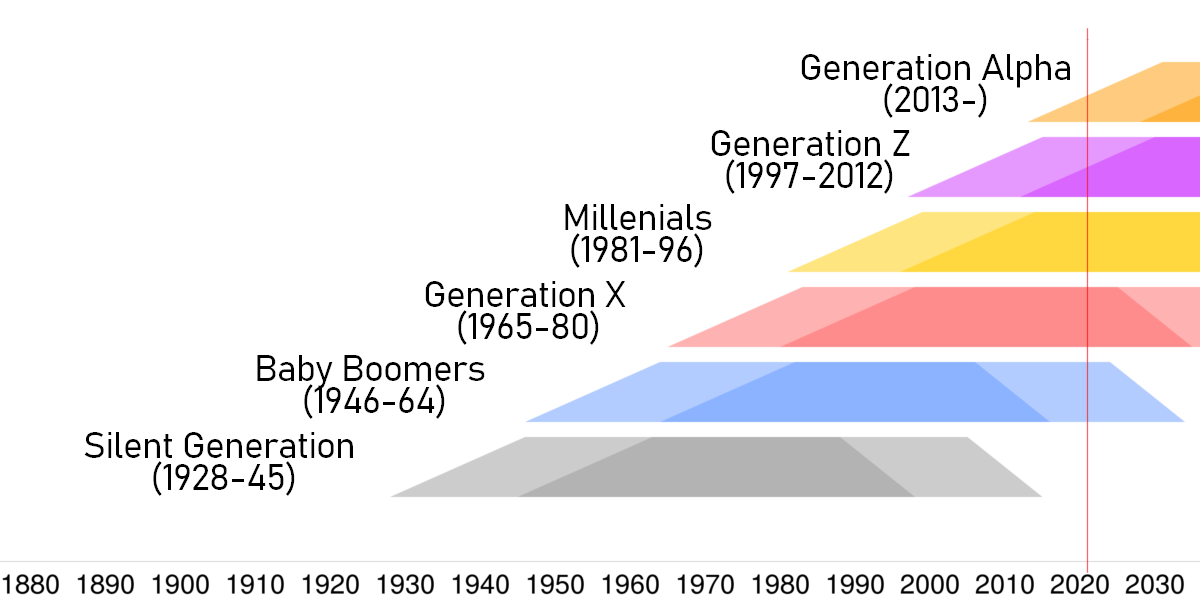
\includegraphics[height=.85\textheight]{logo/generations.png}
    \end{figure}
\end{frame}

\begin{frame}{This thesis}
    \begin{figure}
        \centering%
        \only<1>{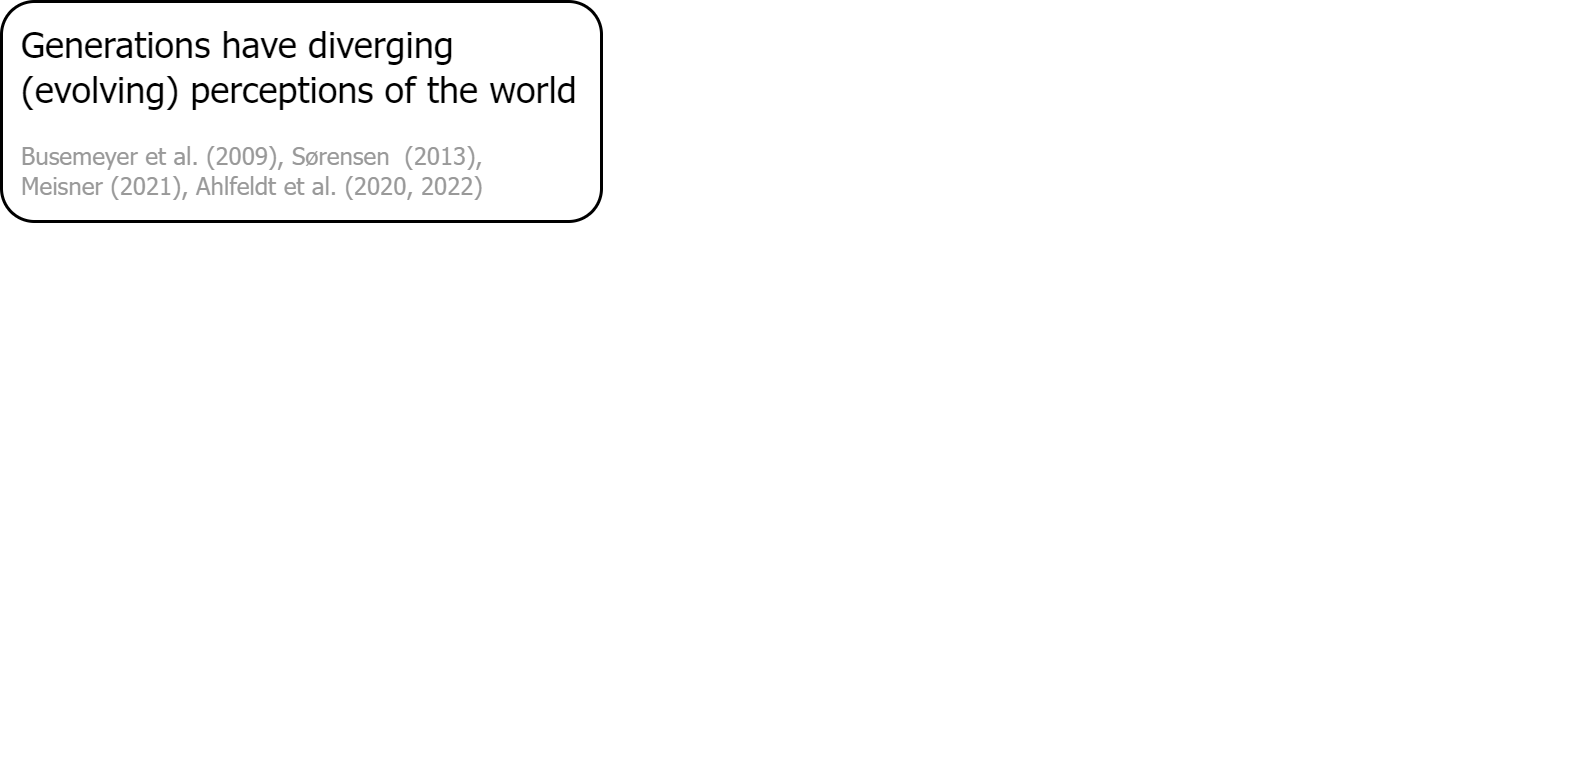
\includegraphics[width=.88\textwidth]{logo/diagram/thesis-diagram-1.png}}\only<2>{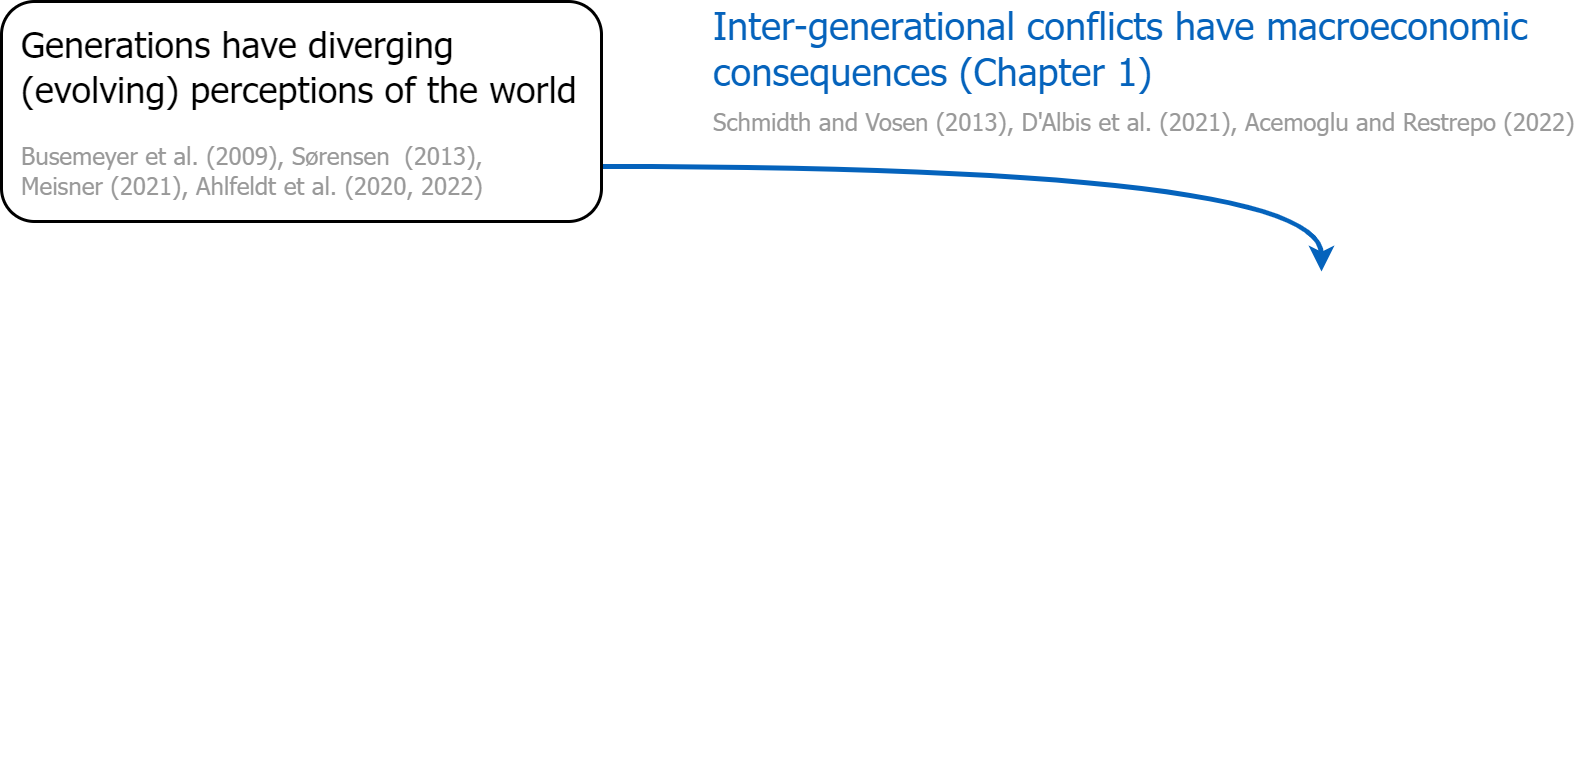
\includegraphics[width=.88\textwidth]{logo/diagram/thesis-diagram-2.png}}%
    \end{figure}
\end{frame}

\AtBeginSection[]
{
  \begin{frame}[plain, noframenumbering]{Outline}
    \begin{NoHyper}\tableofcontents[currentsection]\end{NoHyper}
  \end{frame}
}

\section[Chapter one]{1st Chapter -- Inter-generational conflict and the declining labor share}
\begin{frame}{Motivation}
    \begin{itemize}
        \item \emph{Generations vote differently} (e.g. French presidential elections and Brexit)
        \vspace{1em}\pause
        \item Vote determines public policy which shapes \emph{labor market institutions}
        \vspace{1em}\pause
        \item Change in the \emph{age structure of the population}: Baby-boomer cohorts (1945-1965)
        \vspace{1em}\pause
        \item Decline of the \emph{labor share} in many OECD countries since the beginning of the 1970s
        \vspace{1em}\pause
        \item[$\Rightarrow$] \emph{Is there a coincidence in timing? To what extent the age structure can influence the institutions that play a role in the income allocation?}
    \end{itemize}
\end{frame}

\begin{frame}{This chapter}
    \begin{itemize}
        \item \emph{\textsc{Theory.}} I build an OLG model in which generations with diverging interests vote to determine labor market institutions that matter for wage bargaining
        \vspace{.5em}\pause
        \item[$\Rightarrow$] \emph{Firms shifted away from labor toward capital to respond to young boomers' appropriation of the rents}
        \pause
        \item[$\Rightarrow$] \emph{Expected reversal of the labor share is dampen by the extensive savings of the boomers (i.e. capital deepening)}
        \vspace{1em}\pause
        \item \emph{\textsc{Calibration.}} I calibrate the model for France and the US starting in 1950
        \vspace{.5em}\pause
        \item[$\Rightarrow$] \emph{1 pp. of the labor income share will shift to capital income every 20 years until 2100}
    \end{itemize}
\end{frame}

\begin{frame}{Main contribution}%s}
    \begin{itemize}
        \item Consequences of demographic changes for the allocation between capital and labor income\\
        {\scriptsize\color{OrangeAMSE!75}(\citealt{Schmidt2013Demographic},  \citealt{Albis2021Demographic}, \citealt{Acemoglu2022Demographics})}
        \vspace{.5em}\pause
        \item[$\Rightarrow$] \emph{I introduce a new mechanism based on endogenous labor market institutions}
    \end{itemize}
\end{frame}

\begin{frame}{This thesis}
    \begin{figure}
        \centering
        \only<1>{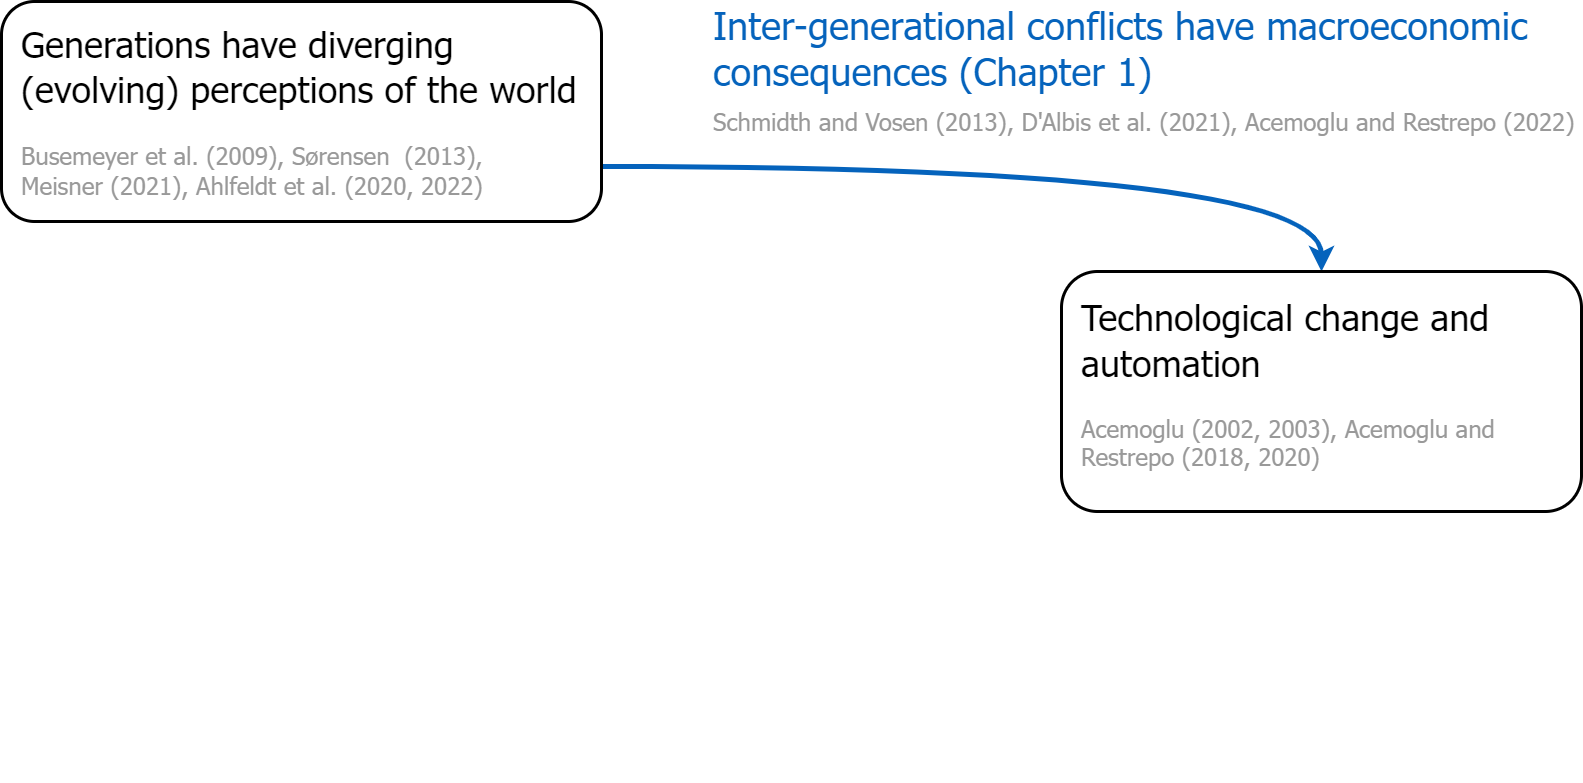
\includegraphics[width=.88\textwidth]{logo/diagram/thesis-diagram-3.png}}\only<2>{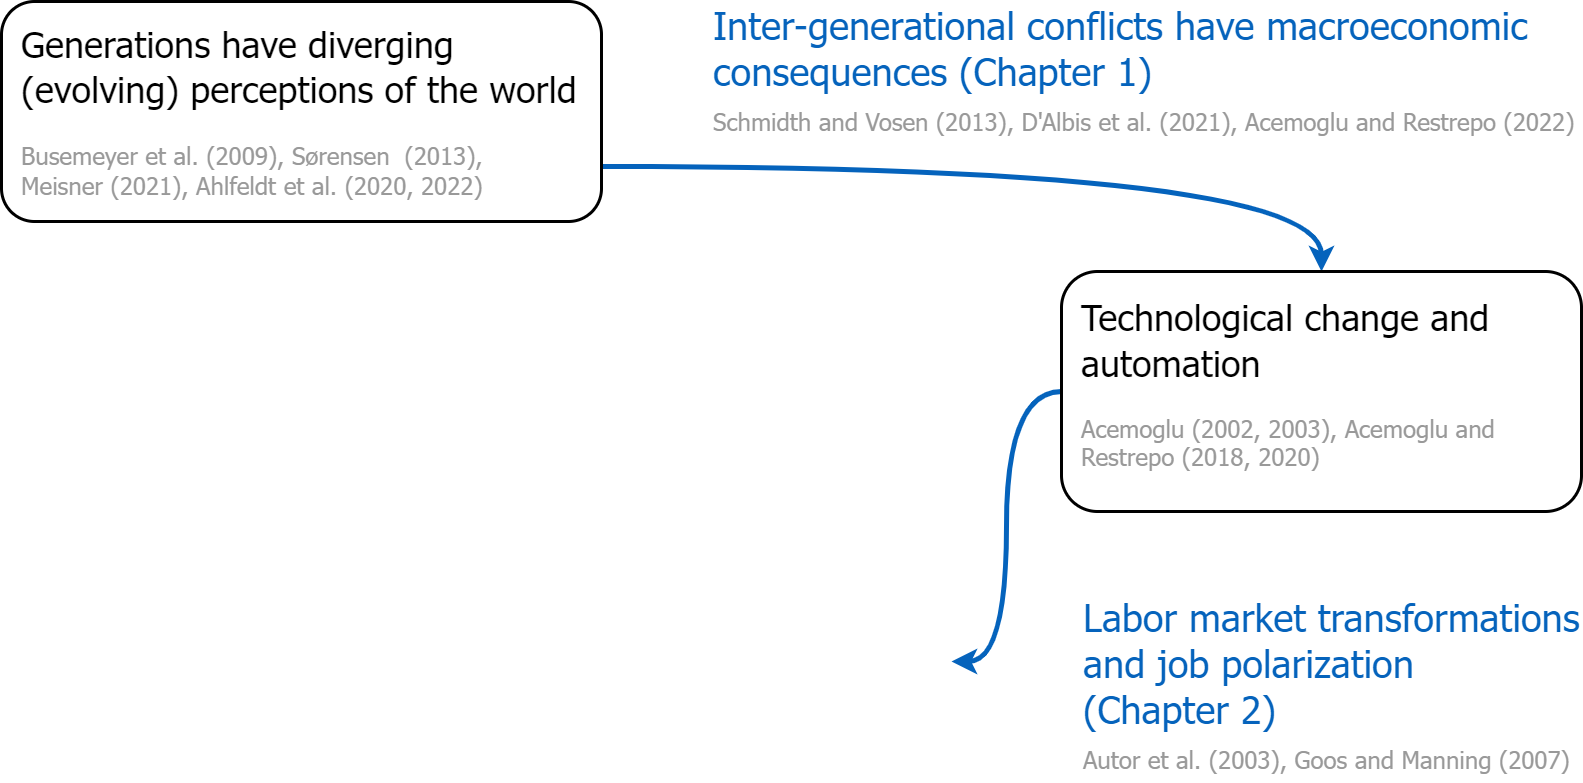
\includegraphics[width=.88\textwidth]{logo/diagram/thesis-diagram-4.png}}
    \end{figure}
\end{frame}

\section[Chapter two]{2nd Chapter -- Spreading the polarization disease: From the labor market to social mobility\\\hfill\textit{(joint research with Cecilia García-Peñalosa and Tanguy van Ypersele)}}
\begin{frame}{Motivation}
    \begin{itemize}
        \item \emph{Increase in job polarization} {\scriptsize \color{OrangeAMSE!75}(\citealt{Autor2003Skill}, \citealt{Goos2007Lousy}, \citealt{Goos2014Explaining}, i.a.)}
        \begin{itemize}
            \item Share in total employment of low- and high-paying occupations has increased at the expense of that of middling occupations
        \end{itemize}
        \vspace{1em}\pause
        \item \emph{Decline in mobility} in the last decades {\scriptsize \color{OrangeAMSE!75}(\citealt{Blanden2007Accounting}, \citealt{Chetty2020Race}, i.a.)}
        \begin{itemize}
            \item Strengthened the link between individuals' origins and their socio-economic outcomes
        \end{itemize}
        \vspace{1em}\pause
        \item[$\Rightarrow$] \emph{Can individuals from less well-off backgrounds still climb the social ladder as the middle rungs become scarce?}
    \end{itemize}
\end{frame}

\begin{frame}{This chapter}
    \begin{itemize}
        \item \emph{\textsc{Theory.}} We develop a model to illustrate how the availability of middling jobs is related to social mobility
        \vspace{1em}\pause
        \item \emph{\textsc{Data.}} We use data on two mature British cohorts born in 1958 and 1970 and exploit the fact that the younger cohort entered a much more polarized labor market
        \vspace{1em}\pause
        \item \emph{\textsc{Empirics.}} We disentangle changes in social mobility that are due to intra- (job-to-job transition) versus inter-generational component (family background)
        \vspace{.5em}\pause
        \item[$\Rightarrow$] \emph{Intra-generational mobility matters for the correlation between parent and child outcomes}
        \pause
        \item[$\Rightarrow$] \emph{Increased differences in \emph{intra-generational mobility} according to family background}
    \end{itemize}
\end{frame}

\begin{frame}{Main contribution}
    \begin{itemize}
        \item Determinants of inter-generational mobility
            \begin{itemize}
                \item Education {\scriptsize\color{OrangeAMSE!75}(\citealt{Blanden2014Education}, \citealt{Blanden2016Educational}, \citealt{Crawford2016Higher}, i.a.)}
                \item Individuals characteristics {\scriptsize\color{OrangeAMSE!75}(\citealt{Chadwick2002Intergenerational}, \citealt{Chetty2020Race})}
                \item Childhood outcomes linked to family background and the quality of neighborhood {\scriptsize\color{OrangeAMSE!75}(\citealt{Heckman2006Effects}, \citealt{Blanden2007Accounting}, \citealt{Chetty2014Land}, i.a.)}
            \end{itemize}
        \vspace{.5em}\pause
        \item[$\Rightarrow$] \emph{We show that intra-generational mobility is essential to understand the link between family background and individuals' outcomes when mature}
    \end{itemize}
\end{frame}

\begin{frame}{This thesis}
    \begin{figure}
        \centering
        \only<1>{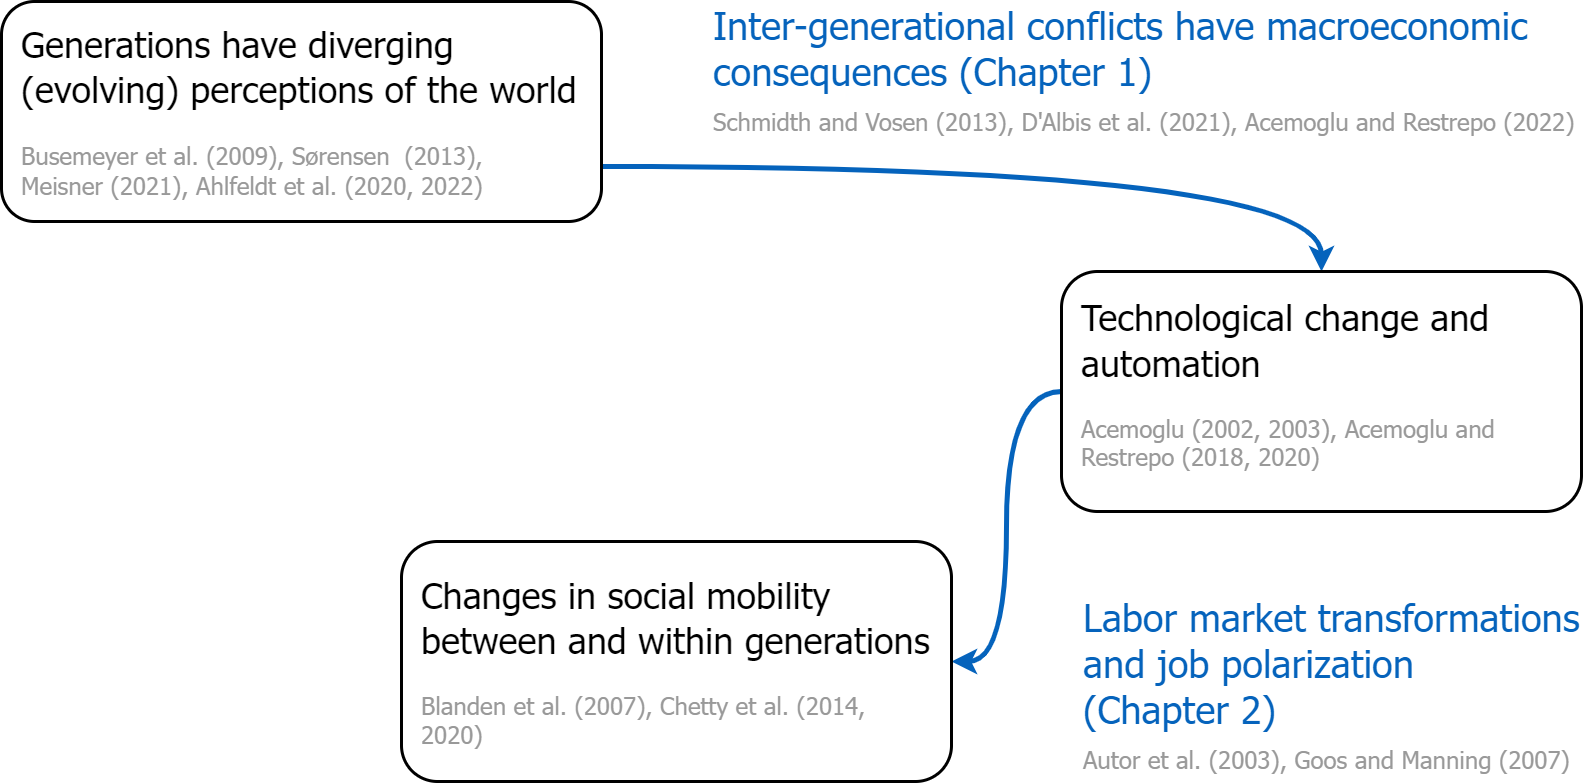
\includegraphics[width=.88\textwidth]{logo/diagram/thesis-diagram-5.png}}\only<2>{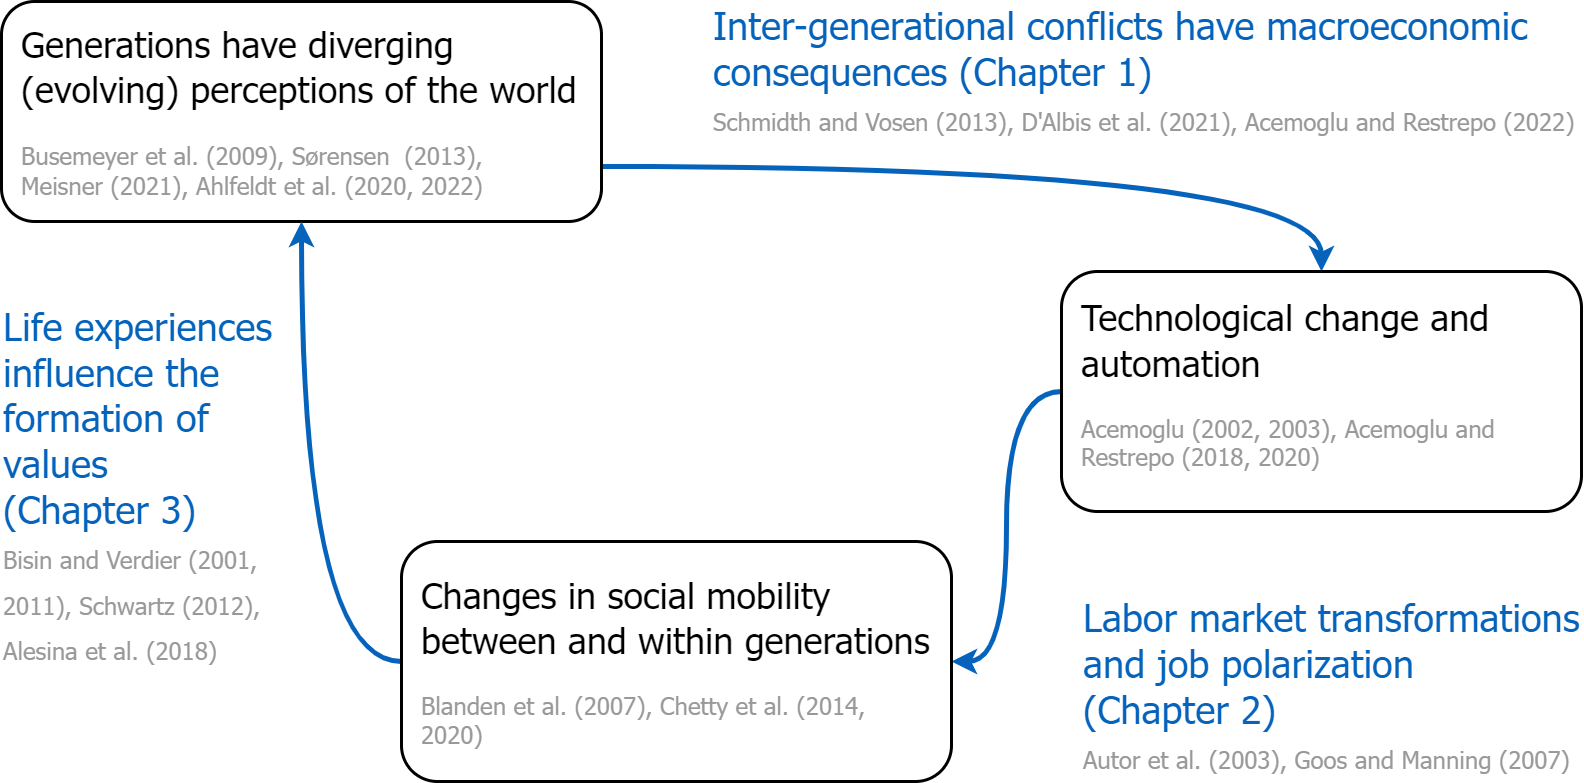
\includegraphics[width=.88\textwidth]{logo/diagram/thesis-diagram-6.png}}
    \end{figure}
\end{frame}

\section[Chapter three]{3rd Chapter -- Spillover effects across values}
\begin{frame}{Motivation}
    \begin{itemize}
        \item \emph{Individuals' values} are personal beliefs about what is important in life
        \vspace{1em}\pause
        \item \emph{Life experiences affect values} (e.g. having a girl $\Rightarrow$ more progressive)
        \vspace{1em}\pause
        \item \emph{Values characterize preferences} that themselves shape individuals' decisions explaining future gaps in economic outcomes (e.g. preference for leisure $\Rightarrow$ effort $\Rightarrow$ wage)
        \vspace{1em}\pause
        \item Prior work has focused on \emph{one particular experience affecting a single value}
        \vspace{1em}\pause
        \item[$\Rightarrow$] \emph{What happens when there is more than one value?}
    \end{itemize}
\end{frame}

\begin{frame}{This chapter}
    \begin{itemize}
        \item \emph{\textsc{Theory.}} I build a model to explain how an agent adjusts her values after a life event based on group identity and cognitive dissonance
        \vspace{.5em}\pause
        \item[$\Rightarrow$] \emph{Shocks to one value that induce a change in group membership will lead to changes in other values (spillover effect)}
        \vspace{1em}\pause
        \item \emph{\textsc{Data.}} I use British cohort data in which I measure individuals' values at several ages
        \vspace{1em}\pause
        \item \emph{\textsc{Empirics.}} I estimate the effect of several life events on values
        \vspace{.5em}\pause
        \item[$\Rightarrow$] \emph{Life events change values throughout the lifecycle and spillover effects across values exist}
    \end{itemize}
\end{frame}

\begin{frame}{Main contribution}
    \begin{itemize}
        \item Existing literature has focused on one particular experience affecting a single value\\
        {\scriptsize\color{OrangeAMSE!75}(\citealt{Piketty1995Social},  \citealt{Mayda2006Against}, \citealt{Fernandez2007Women}, \citealt{Washington2008Female}, \citealt{Alesina2018Intergenerational} i.a.)}
        \vspace{1em}\pause
        \item[$\Rightarrow$] \emph{I show that neglecting the inter-dependence between values underestimates to which extent life experiences affect individuals because this omits the spillover effects}
    \end{itemize}
\end{frame}


\section{Conclusion}
\begin{frame}{Conclusion}
    \begin{itemize}
        \item New evidence of the link between \emph{inter-generational dynamics and the labor market}
        \vspace{1em}\pause
        \item \emph{Intra-generational dynamics} are key in understanding \emph{inter-generational dynamics}
    \end{itemize}
\end{frame}

\begin{frame}{This thesis}
    \begin{figure}
        \centering
        \only<1>{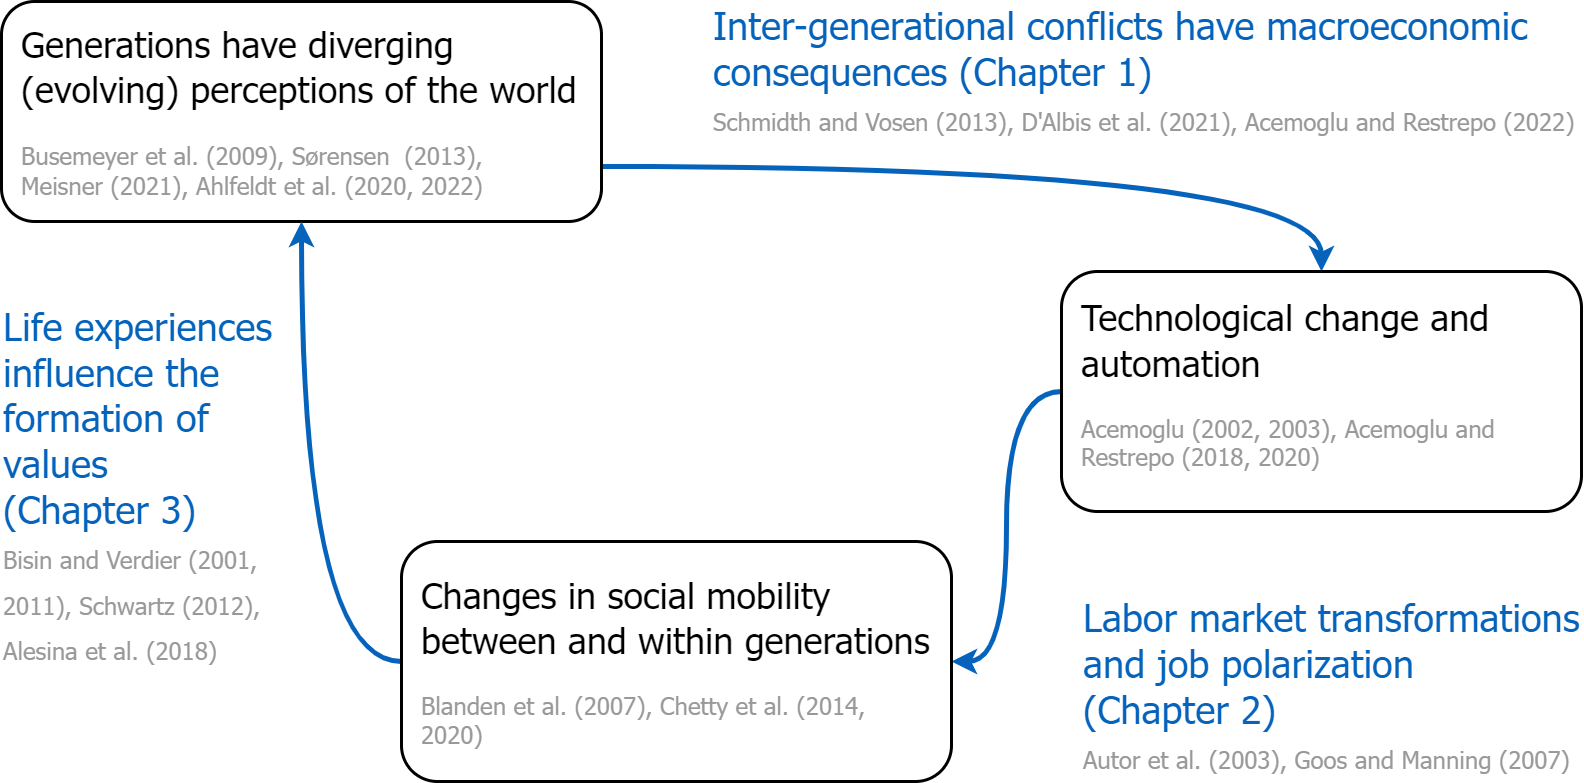
\includegraphics[width=.88\textwidth]{logo/diagram/thesis-diagram-6.png}}\only<2>{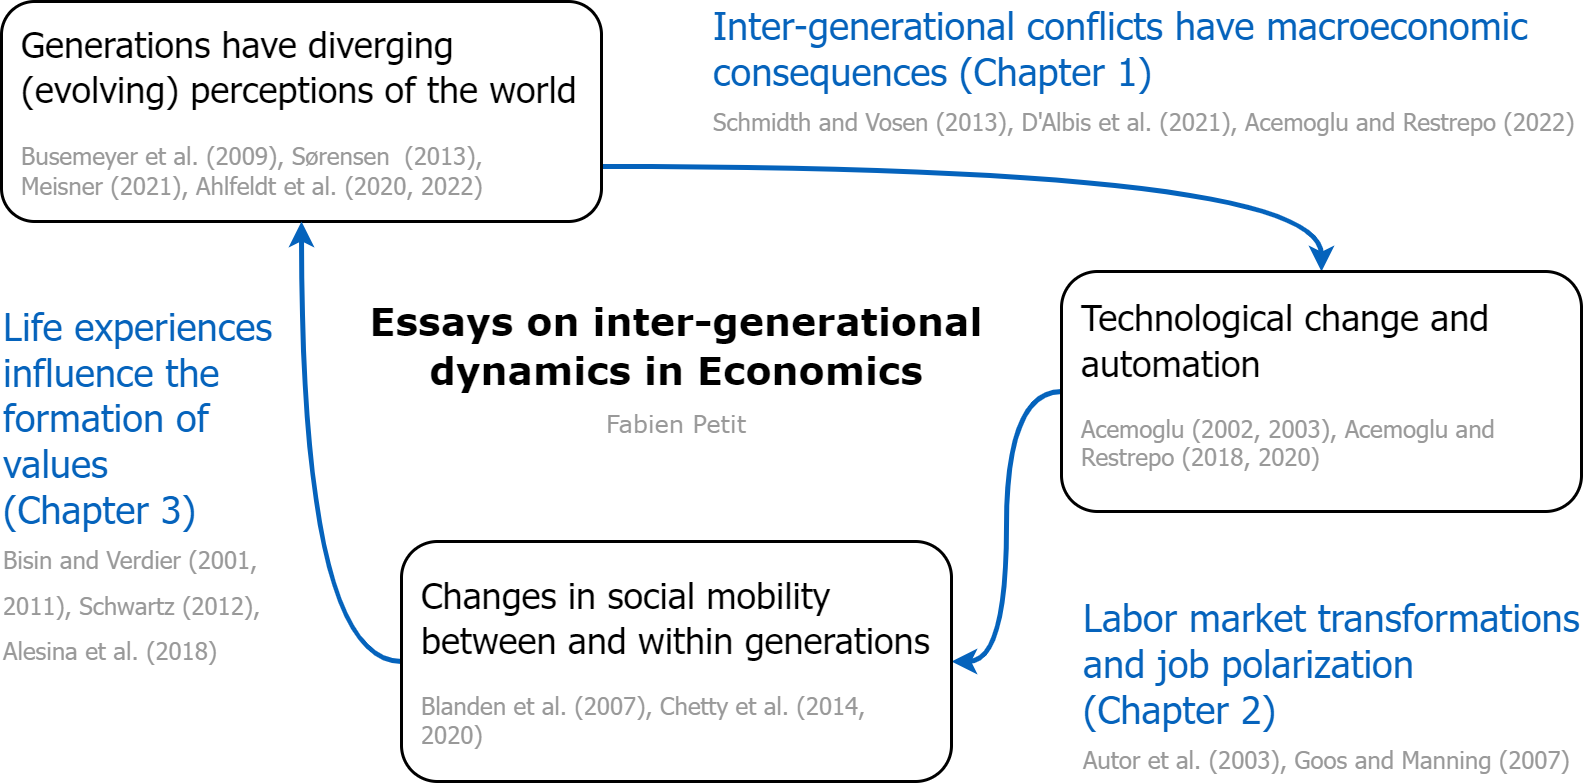
\includegraphics[width=.88\textwidth]{logo/diagram/thesis-diagram-7.png}}
    \end{figure}
\end{frame}

\appendix
	
\begin{frame}<beamer:0>[allowframebreaks]\frametitle{References}
    \footnotesize
    \bibliographystyle{apalike}
    \bibliography{biblio.bib}
\end{frame}


\end{document}